\chapter{Zeitreisen\label{chapter:zeitreisen}}
\lhead{Zeitreisen}
\begin{refsection}
\chapterauthor{Sascha Jecklin und Jonas Gründler}
\section{Einleitung}
	Das Thema Zeitreisen fasziniert den Menschen schon seit Jahrhunderten. Früh entstanden Träume, den Verlauf der Zeit manipulieren zu können. Erste schriftliche und bildliche Belege dafür gab es bereits in der hinduistischen Mythologie und in der buddhistischen Religion. Auch in der modernen Literatur und in der Filmindustrie sind Zeitreisen ein beliebtes Thema. Einige Beispiele dafür sind: 
\begin{itemize}
    \item Time Machine, 1895 von H.G. Wells. Erste literarische Beschreibung einer Zeitreise in die Zukunft mittels Zeitmaschine.
    \item Back to the Future, 1985. Einer der bekannteren Filme über Zeitreisen mit Michael J. Fox.
    \item Star Trek, 1966. Eine Serie mit zahlreichen Ablegern in Film und Büchern. Der Klassiker schlechthin. 
    \item Doctor Who, 1963. Die von BBC produzierte Serie feiert vor allem in den Vereinigten Staaten grosse Beliebtheit. 1996 wurde sogar ein Film produziert. Seit 2005 werden wieder neue Folgen ausgestrahlt.
    \item Interstellar, 2014. Blockbuster vom Batman Produzenten Christoper Nolan. Im Gegensatz zu den meisten anderen Filmen gibt es in diesem Film keine Zeitmaschine. Die Hauptdarsteller erleben Zeitreisen, wenn sie sich in die Nähe eines schwarzen Lochs begeben. Von der Thematik her passt dieser Film gut zu unserer Fragestellung.
\end{itemize}

In diesem Kapitel beschäftigen wir uns mit der mathematischen Beschreibung von Zeitreisen; wie man solche Effekte erreichen kann und ob sie mit heutigen Mitteln erreichbar sind. Zu Beginn soll gezeigt werden, wie man eine Zeitreise mit Hilfe der Eigenzeit beschreibt.

Die Eigenzeit kann als die Zeit verstanden werden, welche für eine mit einem Raumfahrer mitfliegende Uhr vergeht. Die Koordinatenzeit hingegen, entspricht derjenigen Zeit, die für die am Ausgangspunkt der Reise zurückgebliebene Uhr derweil vergangen ist.
Es zeigt sich, dass die beiden Uhren durch Geschwindigkeit und Gravitation tatsächlich unterschiedlich schnell laufen können. Ein besonderes Augenmerk gilt dabei schwarzen Löchern. 

Nach dem wir die nötige Mathematik eingeführt haben, veranschaulichen wir das Ganze mit einer Simulation. Natürlich wollen wir uns auch Gedanken über die Realisierbarkeit machen. Wie sich zeigen wird, scheinen Zeitreisen keine reine Fiktion zu sein. Allerdings sind sie auch nicht in einem Ausmass möglich, wie man es sich vielleicht erhofft.

\section{Was ist eine Zeitreise?}
\rhead{Was ist eine Zeitreise?}
Um diese Frage besser beantworten zu können, starten wir mit einem Gedankenexperiment. Wir stellen uns vor, zwei Autos fahren mit der gleichen Geschwindigkeit aneinander vorbei. Fahren die beiden Autos z. B. 100 km/h, ist die Relativgeschwindigkeit mit der sie sich passieren gerade doppelt so hoch, also 200 km/h. In der klassischen Physik wäre das ein korrektes Ergebnis. In einem zweiten Anlauf sollen beide Fahrer fast Lichtgeschwindigkeit fahren. Spätestens jetzt macht sich ein Fehler bemerkbar. Denn die relative Geschwindigkeit, mit der sich die beiden Fahrzeuge kreuzen, ist nicht etwa doppelte Lichtgeschwindigkeit, sondern einfache Lichtgeschwindigkeit. Denn wir wissen, dass dies die grösste erreichbare Geschwindigkeit ist.

Beide Fahrer behaupten nun aber vehement, ihre eigene Geschwindigkeitsmessung sei korrekt gewesen. Folglich muss es Unterschiede in der Längen- und Zeitmessung geben.

Wie wir in Kapitel \ref{skript:speziell:section:lichtkegel} festgehalten haben, ist dies auch der Fall. Jeder Beobachter misst die gleiche Lichtgeschwindigkeit. Längen- und Zeitmessung müssen folglich angepasst werden. Zeit ist also dehnbar, diese Dehnung nennt man Zeitdilatation. Wir brauchen deshalb die Lorentztransformation aus Kapitel \ref{skript:speziell:section:lorentztransformation}, welche immer auch die Zeit beeinflusst.

\subsection{Die Eigenzeit}
Es gibt also nicht mehr ``die Eine'', allgemeine Zeitmessung für alle Objekte. Jedes Objekt hat seine eigene Zeit, die sogenannte Eigenzeit. Wir müssen also diese angepasste Zeitmessung über den Weg aufsummieren.
Dazu integrieren wir entlang einer Weltenlinie. Wir erhalten für die Eigenzeit
\begin{equation}\label{Eigenzeit}
\tau
=
\int_{}^{}\frac{1}{\gamma}\,dt=\int_{}^{}\sqrt{1-\frac{v^2}{c^2}}\,dt
=
\frac{1}{c}\int_{}^{}\sqrt{g_{\mu\nu}\dot{x}^{\mu}(s)\dot{x}^{\nu}(s)}\,ds.
\end{equation}
Da wir nun für jedes Objekt eine Eigenzeit aufsummieren können, sind wir auch in der Lage, Unterschiede dieser Zeiten anzugeben.
Eine Zeitreise beschreibt daher eine Bewegung durch die Zeit, abweichend von der Koordinatenzeit.

Nicht nur hohe Geschwindigkeiten bringen Änderungen in der Zeitmessung. Wie wir sehen werden, gibt es auch andere Ursachen.

Streng genommen bringt schon jede kleinste Geschwindigkeit eine Änderung der Eigenzeit. Da die praktische Anwendung in diesem Kapitel im Vordergrund steht, interessieren uns natürlich in erster Linie merkliche Unterschiede. Erst doppelt oder sogar zehnmal schneller vergehende Eigenzeiten würden uns Effekte bestätigen, welche man uns in Science Fiction Filmen und Romanen verspricht.

\subsection{Zukunft und Vergangenheit}
Es stellt sich noch die Frage, ob das nun Reisen in die Zukunft oder in die Vergangenheit sind. Dazu folgende Überlegungen:

\subsubsection{Zukunft}
Mit unterschiedlich schnell verlaufenden Eigenzeiten beschreibt man, salopp ausgedrückt, Reisen in die Zukunft oder ``weniger schnelles Altern''. Ein Beobachter $A$ mit halb so schnell verlaufender Eigenzeit wie eine Referenz $B$ wäre quasi in die Zukunft gereist.
Während z. B. für den Beobachter $A$ ganz normal ein Jahr verstrich wären für $B$ zwei Jahre vergangen. $A$ ist somit in die Zukunft gereist. Aus Sicht von $B$ ist $A$ weniger schnell gealtert. Wichtig ist dabei, dass beide älter wurden. Die Zeit hat keine Sprünge gemacht oder ist stehen geblieben. $A$ und $B$ haben beide einen ``normalen'' Verlauf der Zeit erlebt.

\subsubsection{Vergangenheit}
Generell sind Reisen in die Vergangenheit sehr schwierig. Denn dort können Kausalitätsprobleme auftreten. Eine Wirkung folgt nicht mehr zwingend der Ursache. Was z. B. geschieht, wenn ein Zeitreisender seine Entstehung verhindern würde? Diese Frage lässt sich im Moment nicht beantworten. 

Nebst diesen philosophischen Aspekten gibt es auch noch technische Probleme. Selbst wenn sich eine Reise in die Vergangenheit mathematisch korrekt formulieren lassen würde, ist eine praktische Umsetzung momentan undenkbar.

\section{Einfluss von Geschwindigkeit und Gravitation}
\rhead{Einfluss von Geschwindigkeit und Gravitation}
Da wir jetzt wissen, wie wir eine Zeitreise beschreiben können, müssen wir uns nun Gedanken machen, wie wir Zeitdilation erreichen können. Im Wesentlichen gelingt dies durch Geschwindigkeit oder Gravitation. 
\subsection{Geschwindigkeit}
Hohe Geschwindigkeit ist eine Möglichkeit, Zeitdilatationen zu erreichen. Wenn sich eine Person relativ zu einem Bezugssystem schnell bewegt, vergeht für diese Person die Zeit im Vergleich zum Bezugssystem langsamer. Die Differenz wird durch den Lorentzfaktor 
\begin{equation} \label{lorentzfaktor}
\gamma=\frac{1}{\sqrt{1-\displaystyle\frac{v^2}{c^2}}} 
\end{equation}
beschrieben, welcher sich aus der Lorentztransformation herleiten lässt.
Er beschreibt, wie stark die Eigenzeit im Verhältnis zu einem Bezugssystem gedehnt wird. 
Dies ist auch das $\gamma$, welches in der Berechnung der Eigenzeit \eqref{Eigenzeit} vorkommt. 

Die Formel \eqref{Eigenzeit} ist in dieser Form noch nicht sehr anschaulich. Sie zeigt, dass die gewählte Metrik mit den jeweiligen Koordinaten ``multipliziert'' werden muss (Einsteinsche Summenkonvention). Je nach Metrik werden andere Faktoren in die Berechnung mit einbezogen, wie z. B. die Gravitation. Eine solche Metrik werden wir später verwenden.

Durch das Verwenden der Minkowski-Metrik, welche Raum und Zeit miteinander verbindet 
\begin{equation}
    g_{\mu\nu}=
    \begin{pmatrix}
        -1 & 0 & 0 & 0 \\
        0 & 1 & 0 & 0 \\
        0 & 0 & 1 & 0 \\
        0 & 0 & 0 & 1
    \end{pmatrix}
\end{equation}
und der Koordinaten $t, x, y, z$ (Standard-Vierervektor)
\begin{align*}
x^{0}=ct,\qquad x^{1}=x,\qquad x^{2}=y,\qquad x^{3}=z 
\end{align*}
lässt sich eine verständliche Form herleiten.
Aus diesen Koordinaten kann man nun mittels Ableiten die Geschwindigkeiten bilden. Diese werden dann entsprechend der Einsteinschen Summenkonvention multipliziert, sodass folgendes Integral entsteht 
\begin{equation}\label{minkowski}
    \tau
    =
    \frac{1}{c}\int_{}^{}\sqrt{-(-c^2\dot{t}(s)^{2}+\dot{x}(s)^{2}+\dot{y}(s)^{2}+\dot{z}(s)^{2})}\,ds.
\end{equation} 
Dieses stellt nun die Eigenzeitformel auf Basis der Minkowski-Metrik dar.

Wählen wir zur Veranschaulichung eine Bewegung nur in x-Richtung fallen die Koordinaten $y$ und $z$ weg:
\begin{align*}
     t(s)= s,
 	 \qquad x(s)=u\cdot c \cdot s,
     \qquad y(s)=0,
     \qquad z(s)=0 
\end{align*}
Für den Geschwindigkeitsvektor erhalten wir somit:
\begin{align*}
     \dot{t}(s)=1,
     \qquad\dot{x}(s)=u\cdot c,
     \qquad\dot{y}(s)=0,
     \qquad\dot{z}(s)=0
\end{align*}
$c$ stellt die Lichtgeschwindigkeit dar, während $u$ einen Bruchteil von $c$ beschreibt.
Diese Koordinaten in das Integral \ref{minkowski} eingesetzt ergeben
\begin{align*}
\tau
&=
\frac{1}{c}\int_{}^{}\sqrt{-(-c^2\dot{t}(s)^2+\dot{x}(s)^2)}\,ds 
=
\frac{1}{c}\int_{}^{}\sqrt{-(-c^2 +(u\cdot c)^{2}}\,ds\\
&=
\frac{s\sqrt{c^2+(u\cdot c)^{2}}}{c} 
=
s\sqrt{1-\frac{u^2\cdot c^2}{c^2}}.
\end{align*}
Dies stellt eine der einfachsten Formen einer Zeitdilatation dar. Durch die Vereinfachung und das Einsetzen der Werte entsteht also eine Form, welche dem Lorentzfaktor \eqref{lorentzfaktor} oben entspricht.

\subsubsection{Beispiel}
Machen wir ein Beispiel. Wir nehmen eine geradlinige Bewegung mit 20\% Lichtgeschwindigkeit während einer Reise von einer Stunde. Die Parametrisierung sieht dann wie folgt aus:
$s=3600, u=0.2$ 
\[
\begin{aligned}
t(s)&=s, & x(s)&=0.2c \cdot s, & y(s)&=0, & z(s)&=0 \\
\dot{t}(s)&=1, & \dot{x}(s)&=0.2c, & \dot{y}(s)&=0, & \dot{z}(s)&=0
\end{aligned}
\]
Für die Formel \eqref{minkowski} erhalten wir also
\begin{align*}
 \tau
&=
\frac{1}{c}\int_{0}^{3600}\sqrt{-(-c^2\dot{t}(s)^2+\dot{x}(s)^2)}\,ds
=
\frac{1}{c}\int_{0}^{3600}\sqrt{-(-c^2+((0.2c)^2))}\,ds\\
&=
3600\sqrt{1-\frac{(0.2)^2 c^2}{c^2}} 
=
3600\sqrt{1-(0.2)^2}
=
3527.27.
\end{align*}
Bei einer Reise von 3600 Sekunden, sprich einer Stunde, tritt also eine Zeitdilatation von ca. 73 Sekunden auf. Der Reisende ist also eine Minute und 13 Sekunden in die Zukunft gereist.

\subsubsection{Der Lorentzfaktor in Abhängigkeit von $v$}
In Abbildung \ref{skript:zeitreisen:fig:lorentz} sieht man den Zusammenhang zwischen Geschwindigkeit und Lorentzfaktor als Graph. Obiges Beispiel und die Abbildung zeigen, dass eine relevante Zeitdilatation erst bei sehr hohen Geschwindigkeiten erreicht wird. Um wirklich grosse Zeitdilatationen zu erreichen, braucht man annähernd Lichtgeschwindigkeit. Wie bald ersichtlich wird, stellt dies bei der Realisierung ein Problem dar.
\begin{figure}[H]
   \centering
   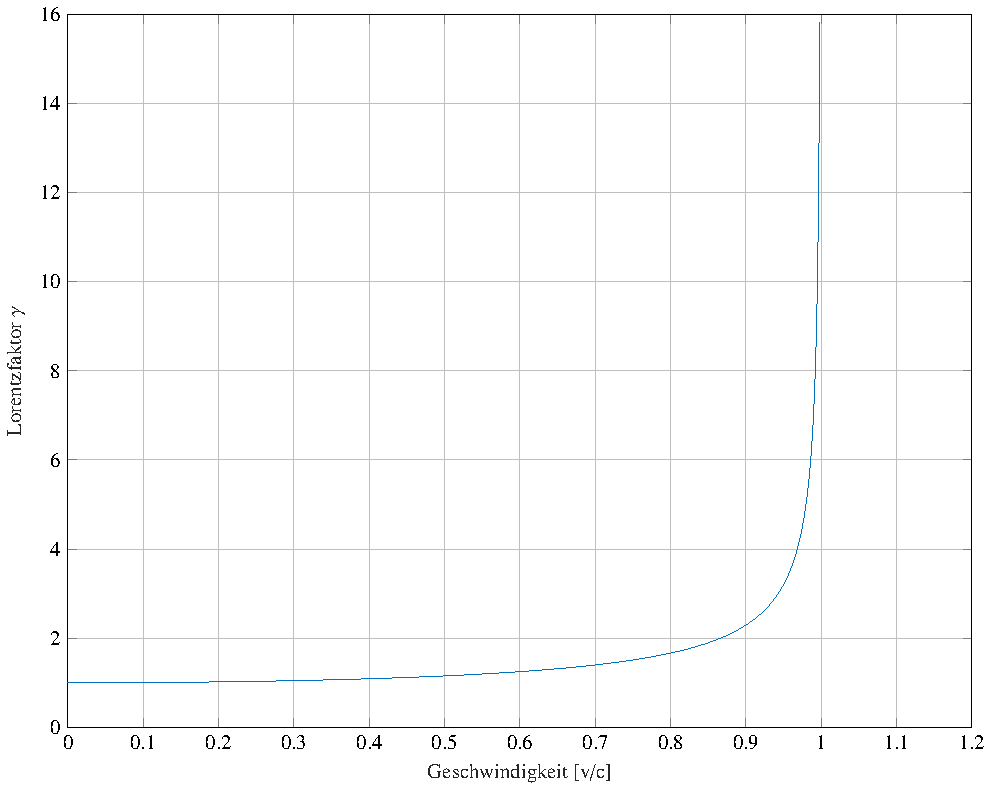
\includegraphics[width=12cm]{zeitreisen/tikz/lorentz.pdf}
   \caption{Änderung des Lorentzfaktors in Abhängigkeit der Geschwindigkeit}
   \label{skript:zeitreisen:fig:lorentz} 
\end{figure}
\subsection{Gravitation} \label{Gravitation}
	Der Einfluss der Gravitation auf die Zeit muss noch genauer untersucht werden. Einstein hat erkannt, dass die Gravitation durch eine Krümmung des Raumes beschrieben werden muss. Erkennen lässt sich die Gravitation z. B. an der Erdbeschleunigung. Alles wird mit $g=9.81\frac{\text{m}}{\text{s}^2}$ in Richtung Erdmittelpunkt beschleunigt. Die Gravitationskraft $F$ lässt sich nach dem zweiten Newtonschen Gesetz als $F=m\cdot a$ schreiben. Wenn dieser Term nun in die Formel für Gravitation eingesetzt wird, lässt sich $m$ wegkürzen: 
	\begin{align*}
		m\cdot a = \frac{KMm}{r^2} \Leftrightarrow a=\frac{KM}{r^2} 
	\end{align*}
    Das bedeutet, dass die Beschleunigung nicht vom der Masse des Objektes abhängt. Mit der Masse der Erde in $M$ eingesetzt, der Gravitationskonstanten $K$ und dem Radius der Erde $r$ ergibt sich sogleich die bekannte Beschleunigung $g$.
    
	Dieser Effekt lässt sich leider nicht oft beobachten, da beispielsweise eine Feder langsamer fällt als ein Stein. Dies liegt jedoch nicht an der Gravitation, sondern am Luftwiderstand der Objekte. Im luftleeren Raum würden Stein und Feder gleich schnell fallen. Schwere Objekte werden also gleich stark Richtung Erdmittelpunkt beschleunigt wie leichte.
	
	\subsubsection{Koordinatentransformationen}
    Die Ursachen für Zeitdilatationen müssen noch in Transformationen berücksichtigt werden. 
	Die Gleichungen 
	\begin{equation}\label{skript:gravitation:beschleunigt}
	\left.
	\begin{aligned}
	t'&=t\\
	x'&=x+\frac12gt^2
	\end{aligned}
	\right\}
	\qquad
	\Leftrightarrow
	\qquad
	\left\{
	\begin{aligned}
	t&=t'\\
	x&=x'-\frac12gt'^2
	\end{aligned}
	\right.
	\end{equation}
    sind zwar eine Koordinatentransformation jedoch keine Lorentztransformation, denn sie enthalten keine Minkowski-Metrik. Mit ihnen lässt sich der Einfluss der Gravitation auf die Zeit nicht berechnen. 
    In der Transformation \ref{skript:gravitation:beschleunigt} wird ein frei fallendes Koordinatensystem in ein mit der Erde verbundenes Koordinatensystem umgewandelt. Die x-Koordinate ist also nicht mehr frei, der Einfluss der Erdbeschleunigung muss einberechnet werden.
	Das $t'$ entspricht immer noch $t$ obwohl eine Transformation durchgeführt wurde. Obwohl die Erdgravitation miteinbezogen wurde, hat sich $t$ nicht verändert.
	
	Der Ansatz $ -c^2dt^2 + dx^2 + dy^2 + dz^2$ genügt also nicht mehr. Wir müssen also Metriken und Transformationen zulassen, welche von der Minkowski-Metrik und der Standardtransformation abweichen.
	
	\subsubsection{Metriken}\label{skript:chapter:zeitreisen:metriken}
	Doch welche Metrik beinhaltet den Einfluss der Gravitation auf die Zeit? 
	Da der Raum durch die Gravitation gekrümmt wird, benötigen wir eine Metrik für die Längen- und Zeitmessung, welche gravitative Effekte miteinbezieht.
	Zum Glück kennen wir bereits eine solche Metrik. Die Schwarzschild-Metrik eignet sich bestens dazu, denn sie beschreibt die Raumkrümmung um massereiche Objekte. Wir werden sie später auf ein schwarzes Loch anwenden. 

	\section{Realisierbarkeit}
    \rhead{Realisierbarkeit}
    Theoretisch sind Zeitreisen also umsetzbar. Nun gilt es zu prüfen, inwiefern so etwas in der Praxis möglich ist. Es gibt mehrere Probleme, die eine Zeitreise verhindern können.
    
    Betrachten wir zuerst grosse Geschwindigkeiten. Wie wir in Abbildung \ref{skript:zeitreisen:fig:lorentz} bereits gesehen haben, treten die gewünschten Effekte erst bei annähernd Lichtgeschwindigkeit auf. Ab $0.99c$ beginnt der Faktor $\gamma$ stark zu wachsen und die Zeitdilatation würde für uns akzeptable Werte erreichen.
    Doch wie lässt sich diese Geschwindigkeit überhaupt erreichen?
    
    \subsubsection{Energie}\label{skript:chapters:zrirtreisen:energie}
    Wie aus der Physik bekannt ist, berechnet sich die kinetische Energie eines Objekts aus $E_{\text{kin}}=\frac{1}{2}mv^2$. Doch der Faktor $c^2$ lässt die kinetische Energie auch für verschwindend kleine Massen ins Unerreichbare schnellen.
    
    Momentan spekuliert man darüber, ob es möglich ist, kleine Sonnensegel mittels Laserstrahlen auf 20\% Lichtgeschwindigkeit zu beschleunigen und diese dann Richtung Proxima-Centauri (nächste Sonne ausserhalb unseres Sonnensystems) zu schiessen. Dass ein Mensch und sein Fortbewegungsmittel also beinahe Lichtgeschwindigkeit erreichen können ist momentan undenkbar.
    
    Das bedeutet also, mittels Geschwindigkeit können in naher Zukunft keine merklichen Zeitdilatationen erreicht werden. Auch wenn der Effekt in gewissen Präzisionsanwendungen berücksichtigt werden muss, ist er für unserer Zwecke zu schwach. Bleibt zu hoffen, dass die Gravitation bessere Resultate bringt. 
    
    \subsubsection{Massereiche Objekte}
    Um also eine Zeitdilatation zu erreichen, müssen wir auf die Gravitation ausweichen. Betrachten wir als erstes die Erde. Die Gravitation der Erde beeinflusst die Zeit in GPS-Satelliten bereits derart, dass die resultierenden Fehler mathematisch herausgerechnet werden müssen. Im Kapitel \ref{chapter:gps} ergibt sich für Satelliten eine Abweichung von $45.713 \frac{\mu\text{s}}{\text{d}}$. Was für die Genauigkeit von GPS-Systemen grosse folgen hat, reicht für eine merkliche Zeitreise aber noch nicht aus.
    %label noch nicht online 
    
    Da der Effekt also zu klein für eine wirkliche Zeitreise ist, lässt sich die gleiche Rechnung mit der Sonne machen. Schnell wird klar, dass selbst die grössten Sterne zu wenig Masse haben, um eine nennenswerte Zeitdilatation zu verursachen. Wir müssen also noch schwerere Objekte betrachten. Objekte an denen man im besten Fall auch nahe vorbei fliegen kann. 
     
    Das Ergebnis aus diesem Ausschlussverfahren sind deshalb, als letzte Option, schwarze Löcher. Die sogenannten ``Stellar-size black holes'' kommen relativ häufig vor, besitzen aber nur einige Sonnenmassen. Wir benötigen supermassive schwarze Löcher. Und davon gibt es in unserer Galaxie lediglich eines.
    
     Von unserer Position aus gesehen, ist das nächste grosse schwarze Loch Sagittarius A*, welches sich im Zentrum unserer Galaxie befindet. Es hat ca. vier Millionen Sonnenmassen. Dieses sogenannte supermassive schwarze Loch sollte den Anforderungen genügen. Unsere Simulationen werden zeigen, dass sich mittels Sagittarius A* tatsächlich eine merkliche Zeitdilatation erreichen lässt.
    
    \subsection{Reise}
    Doch hier beginnen auch neue Probleme. Sagittarius A* ist 26000 Lichtjahre von uns entfernt. Das bedeutet, selbst das Licht benötigt 26000 Jahre, bis es dort ankommt. Die grosse Hoffnung ist, dass wir durch eine hohe Fluggeschwindigkeit und die daraus resultierende Zeitdilatation die Eigenzeit an Bord des Raumschiffes verkürzen können. 
    Doch wie bereits zuvor ersichtlich wurde, lässt sich eine für unsere Zwecke ausreichende Zeitdilatation erst mit sehr hohen Geschwindigkeiten erreichen. Wir haben also das gleiche Problem. Die Reise dauert zu lange, da für uns eine Geschwindigkeit nahe der Lichtgeschwindigkeit momentan undenkbar ist.
    Hier eine Beispielrechnung, in welcher wir mit einer Geschwindigkeit von $0.5c$ fliegen.
	\begin{align*}
	\tau
	&= 
	\int_{}^{26000}\frac{1}{\gamma}dt=\int_{}^{26000}\sqrt{1-\frac{v^2}{c^2}}\,dt
	= 
	\frac{1}{c}\int_{0}^{26000}\sqrt{-(-c^2+(0.5c)^2)}\,ds\\
	&=
	\biggl[s\sqrt{1-\frac{(0.5c)^{2}}{c^2}}\biggr]_0^{26000}
	=
	22516.7
	\end{align*}
	Wir benötigen für die Strecke also ca. 22500 Jahre.
	Folgende Tabelle zeigt andere Eigenzeiten im reisenden Raumschiff bei verschiedenen Geschwindigkeiten:
    \begin{table}[H]
         \begin{center}
            \begin{tabular}{ | l | l |}
            \hline
            Geschwindigkeit & Eigenzeit im Raumschiff \\ \hline
            $20\%c$ & 25474.5 Jahre \\ 
            $50\%c$ & 22516.7 Jahre \\
            $80\%c$ & 15600 Jahre \\ 
            $99\%c$ & 3667.75 Jahre \\ 
            $99.99\%c$ & 367.686 Jahre \\ 
            $99.9999\%c$ & 36.76 Jahre \\ 
            $99.999999\%c$ & 3.6 Jahre \\ \hline
             \end{tabular}
        \end{center}
    \caption{Eigenzeiten auf der Reise zu Sagittarius A* in Abhängigkeit der Geschwindigkeit.}
    \label{table:eigenzeiten}
    \end{table}
    \noindent
	Wie die Tabelle \ref{table:eigenzeiten} zeigt, würde auch ein Flug mit $0.99c$ noch viel zu lange dauern. 
	Die Eigenzeit im Raumschiff beträgt zwar nur noch einen Bruchteil der Koordinatenzeit, jedoch ist es trotz dieser Zeitersparnis nicht möglich, bei einer normalen Lebenserwartung, das Ziel zu erreichen.
    
	Wir müssen mit unserem Projekt also warten, bis mit Raumschiffen annähernd Lichtgeschwindigkeit erreicht werden kann. Dafür muss auch noch das oben genannte Energieproblem gelöst werden (Abschnitt \ref{skript:chapters:zrirtreisen:energie}). Es muss ein Treibstoff mit grosser Energiedichte gefunden werden, sodass nicht riesige Mengen an Treibstoff mit befördert werden müssen. Dies würde die Masse des Raumschiffes zusätzlich erhöhen und dadurch auch wieder die benötigte Energie vergrössern: Ein Teufelskreis.
    
	Wir verschieben unser Projekt also ins Hypothetische und stellen uns vor, wir wären bereits da.
	
	\subsection{Am Ziel\dots Was nun?}
	Wenn wir nun also diese Reise auf uns genommen haben und Sagittarius A* wirklich erreichen, eröffnen sich uns zwei Möglichkeiten:
	\begin{itemize}
		\item wir fliegen eine gesteuerte Bahn
		\item wir lassen uns ``fallen''
	\end{itemize}
	In den folgenden Abschnitten werden die Vor- und Nachteile der jeweiligen Methoden beschrieben.
	
	\subsubsection{Eine gesteuerte Bahn}
	Eine gesteuerte Kreisbahn um das schwarze Loch bringt die besten Resultate, da wir eine Kreisbahn sehr nahe am Ereignishorizont wählen können. Denn je näher und länger wir uns am Ereignishorizont befinden, desto stärker sind die Auswirkungen auf die Zeit. 
    
	Um jedoch einen konstanten und nahen Orbit am schwarzen Loch zu fliegen, muss das Raumschiff in der Lage sein, der Gravitation zu widerstehen, um den Ereignishorizont nicht zu überschreiten. Das liesse sich auf zwei Arten erreichen. Entweder mittels einer hohen Geschwindigkeit, bei welcher die Fliehkraft des Raumschiffs der Gravitation entgegenwirkt, oder mittels Steuerdüsen. 
	Beide Methoden benötigen sehr viel Energie, und sind deshalb keine wirkliche Option. Die Hin- und Rückreise würden bereits einen grossen Teil des Treibstoffs beanspruchen.
	\subsubsection{Wir lassen uns ``fallen''}
	
	Die zweite Möglichkeit wäre, dass wir uns, in der Nähe des schwarzen Lochs ``fallenlassen''. Wir bewegen uns dann auf einer Bahn um das schwarze Loch  ohne äussere Krafteinwirkung. Dadurch sparen wir uns natürlich einiges an Treibstoff, da wir den immensen Kräften nicht gegensteuern müssen. 
    
    Je nach Anfangsgeschwindigkeit und Abstand können so verschiedene Bahnen erreicht werden. Geschwindigkeit, Richtung und Abstand vom schwarzen Loch stellen bei der Ankunft also gerade die Anfangsbedingungen dar. Vom Absturz in den Ereignishorizont bis zu einer Bahn, auf der wir dem Gravitationstrichter des schwarzen Lochs entkommen und uns in die Weiten des Weltalls verabschieden, ist alles möglich. Beides sind jedoch eher unangenehme Szenarien. Für möglichst grosse Zeitreisen ist es natürlich erstrebenswert, lange und nahe um das schwarze Loch zu kreisen.
	
	Wie findet man also eine Bahn, möglichst nahe dem schwarzen Loch, ohne dass weitere Steuerenergie verwendet werden muss?
    Eine solche Bahn ohne äussere Krafteinwirkung entspricht einer Geodäte. Mit den passenden Anfangsbedingungen können wir die Geodätengleichungen aufstellen, welche eine solche Bahn beschreiben. Durch das Lösen der Gleichung erhalten wir dann auch die Eigenzeit. An der Abweichung zur Koordinatenzeit erkennen wir schlussendlich, wie effizient unsere Zeitreise war.
    In Kapitel \ref{skript:chapter:zeitreisen:simulation} rechnen wir das Ganze in einer Simulation durch, mit der wir sehen können, wie viel Zeit sich wirklich einsparen lässt.
	
	\section{Umsetzung mittels Geodäten}
    \rhead{Umsetzung mittels Geodäten}
	Mit den Geodäten lassen sich nun physikalisch korrekte Bahnen um ein schwarzes Loch berechnen. Sie beschreiben im allgemeinen den kürzesten Weg zwischen zwei Punkten. In diesem Fall sind die Geodäten jedoch anders zu interpretieren. Sie beschreiben nicht den kürzesten Weg, sondern den Weg, welcher unser Raumschiff ohne weitere Krafteinwirkung nehmen wird.
	Zur Berechnung der Geodäten benötigen wir:
	\begin{itemize}
		\item die Geodätengleichungen (siehe unter \ref{skript:chapter:zeitreisen:geodaetengl})
		\item die Schwarzschild-Metrik (siehe unter \ref{skript:chapter:zeitreisen:schwarzschildmetrik})
		\item die Christoffelsymbole (siehe unter \ref{skript:chapter:zeitreisen:christoffel})
	\end{itemize}

	\subsection{Die Geodätengleichung}\label{skript:chapter:zeitreisen:geodaetengl}
	Wie bereits erwähnt, beschreiben die Geodäten einen Weg ohne äussere Krafteinwirkung. In der in Kapitel \ref{skript:chapter:geodaeten} vorgestellten Geodätengleichung
	\begin{equation}
	\ddot{x}^{\alpha} + \Gamma^{\alpha}_{\mu\nu}\dot{x}^{\mu}\dot{x}^{\nu} = 0
	\end{equation}
    sehen wir, dass sich die Beschleunigungen und die Christoffelsymbole gerade zu $0$ addieren.
	Stellen wir die Gleichung um	
	\begin{equation}\label{equation:geodaetengleichung}
	\ddot{x}^{\alpha} = -\Gamma^{\alpha}_{\mu\nu}\dot{x}^{\mu}\dot{x}^{\nu}
	\end{equation}
	lässt sich daraus interpretieren, dass die Beschleunigungen zu jedem Zeitpunkt ein Produkt, aus den $\Gamma$ mit den jeweiligen ersten Ableitungen sind.
    
	Diese $\Gamma$ sind die Christoffelsymbole und werden auch Zusammenhangskoeffizienten genannt. Sie beschreiben kovariante Ableitungen und Geodäten auch ohne Verwendung einer Metrik. Für die Formel \eqref{equation:geodaetengleichung} können wir also die im Kapitel Gravitation \ref{Gravitation} bereits erwähnte Schwarzschild-Metrik einsetzten.	
	 
	Die Schwarzschild-Metrik in der in diesem Buch verwendeten Form setzt Kugelkoordinaten voraus. Wir können nun also die einzelnen Koordinaten ausschreiben 	
	\begin{equation}\label{skript:chapter:zeitreisen:geodaeten4dim}
	\begin{aligned}
	\ddot{t}(s) = -\Gamma^{1}_{\mu\nu}\dot{x}^{\mu}\dot{x}^{\nu}\\
	\ddot{r}(s) = -\Gamma^{2}_{\mu\nu}\dot{x}^{\mu}\dot{x}^{\nu}\\
	\ddot{\vartheta}(s) = -\Gamma^{3}_{\mu\nu}\dot{x}^{\mu}\dot{x}^{\nu}\\
	\ddot{\varphi}(s) = -\Gamma^{4}_{\mu\nu}\dot{x}^{\mu}\dot{x}^{\nu}	
	\end{aligned}
	\end{equation}
    und es entsteht ein Differentialgleichungssystem 2. Ordnung.

	\subsection{Schwarzschild-Metrik}\label{skript:chapter:zeitreisen:schwarzschildmetrik}
	
	Die von Karl Schwarzschild gefundene Metrik ist eine Lösung der Einsteinschen Feldgleichungen. Sie wurde nur wenige Monate nach der Vorstellung der Feldgleichungen gefunden und stellt eine vergleichsweise einfache Lösung dar. 
    
    Sie geht davon aus, dass das schwarze Loch nicht rotieren und auch keine Ladung besitzt. Dadurch nehmen wir einerseits einen Fehler in Kauf, andererseits hält sich der rechnerische Aufwand in Grenzen. Um diese weiteren Effekte miteinzubeziehen müsste man die Kerr- oder die Kerr-Newman Metrik verwenden. Das Rechnen mit diesen Metriken ist um ein Vielfaches komplizierter. Der Ansatz ist genau der gleiche. Allerdings entstehen viel mehr Terme welche numerisch auch schwieriger zu handhaben sind. Die Schwarzschild-Metrik genügt, um zu überprüfen, ob merkliche Zeitreisen überhaupt möglich sind. Deshalb beschränken wir uns auf sie.
    
	In Matrixdarstellung
	\begin{equation}\label{equation:schwarzschild}
	g_{\mu\nu}=
	\begin{pmatrix}
	-\biggl(-1- \displaystyle \frac{r_{g}}{r}\biggr) & 0 & 0 & 0 \\
	0 & \frac{\displaystyle 1}{\displaystyle1-\frac{r_{g}}{r}} & 0 & 0 \\
	0 & 0 & r^{2} & 0 \\
	0 & 0 & 0 & r^{2}\sin^{2}(\vartheta)
	\end{pmatrix}
	\end{equation}
	sieht man, dass wie bei der Minkowski-Metrik die Zeitkoordinate negativ ist. Dies entspricht der klassischen Raum-Zeit-Signatur. Die Erklärung dazu ist im Kapitel \ref{skript:speziell:section:lichtkegel} zu finden.
    
	Mit der Parametrisierung
	\begin{align*}
	x^{0}=c \cdot t, \qquad
	x^{1}=r \qquad,
	x^{2}=\vartheta, \qquad
	x^{3}=\varphi
	\end{align*}
    erhält man ein um die Zeit erweitertes Kugelkoordinatensystem.
    
	Ausmultipliziert lässt sie sich dafür in Zeilenform
	\begin{equation}
	ds^2
	=
	-\biggl(1-\frac{r_g}r\biggr)c^2\,dt^2
	+
	\frac{1}{\displaystyle 1-\frac{r_g}r}\,dr^2 
	+
	r^2d\vartheta^2 
	+ 
	r^2\sin^2(\vartheta)d\varphi
	\end{equation}
	darstellen, welche auch gleich die Längenmessung im betrachteten Raum darstellt.
	
	\subsubsection{Bedeutung von $r_{g}$ und $r$}
 	Der Ereignishorizont 
     \begin{equation} \label{Gravitationsradius}
     r_{g}= \frac{2MG}{c^2}
     \end{equation}
     oder auch Gravitationsradius genannt, stellt in der allgemeinen Relativitätstheorie eine Grenzfläche dar. Er beschreibt die Entfernung, ab welcher das Licht nicht mehr aus dem Gravitationsfeld des schwarzen Lochs entkommen kann. Teilchen, welche den Ereignishorizont passiert haben, können diesen nicht mehr verlassen. Alle Teilchen oder Objekte die den Ereignishorizont passieren, werden unweigerlich ins Zentrum stürzen. 
	
	Der Gravitationsradius der Erde beträgt etwa 8.8 mm. Wenn wir die Erde auf unter 8.8 mm Radius komprimieren könnten, würde sie zu einem schwarzen Loch werden.
    
    Das $r$, welches in der Matrix vorkommt ist der Radius. Also der Abstand vom Raumschiff zum schwarzen Loch. Es stellt sich die Frage, wie man denn von einem Abstand zum schwarzen Loch sprechen kann. Bis zum Ereignishorizont ist eine Längenmessung noch möglich, aber für die Teilstrecke innerhalb ist dies nicht der Fall. Man kann sich das so vorstellen, dass man von sich aus einen langen Massstab zum schwarzen Loch führt. Sobald er den Ereignishorizont überquert, wird er unweigerlich in die Länge gezogen.
    
    Durch einen Trick lässt sich dieses Dilemma umgehen. Der Umfang, den man auf einer Kreisbahn um das schwarze Loch hat, lässt sich messen. Durch eine Division mit $2\pi$ erhält man den Radius.
	
	\subsection{Christoffelsymbole}\label{skript:chapter:zeitreisen:christoffel}
	
	Die Berechnung der Christoffelsymbole aus der Schwarzschild-Metrik ist kompliziert und sehr rechenaufwändig. Wir beschränken uns hier auf die Berechnung. Die Herleitung wird in Kapitel \ref{skript:chapter:geodaeten} ausführlich beschrieben. 
	
	Theoretisch würden für ein vierdimensionales Koordinatensystem $4^{3}$ also $64$ Christoffelsymbole entstehen. Der grösste Teil der Symbole wird allerdings zu $0$ und fällt somit weg. Das vereinfacht auch die Geodätengleichungen um viele Terme. 
	Für die Schwarzschild-Metrik entstehen nach einer Berechnung mit MAXIMA folgende Terme:
	
	\begin{align*}
	\Gamma^0_{01}
	&=
	\frac{1}{1-\displaystyle\frac{r_g}{r}}
	\frac{r_g}{r}
	\frac{1}{2r}
	\\
	\Gamma^1_{00}
	&=
	\biggl(1-\displaystyle\frac{r_g}{r}\biggr)
	\frac{r_g}{r}
	\frac{1}{2r}
	&
	\Gamma^1_{11}
	&=
	-\frac1{1-\displaystyle\frac{r_g}{r}}
	\frac{r_g}{r}
	\frac{1}{2r}
	&
	\Gamma^1_{22}
	&=
	r_g-r
	&
	\Gamma^1_{33}
	&=
	r_g-r
	\\
	\Gamma^2_{12}
	&=
	\frac1r
	\\
	\Gamma^3_{13}
	&=
	\frac1r
	\end{align*}
	Terme welche $\dot{\vartheta}(s)$ enthalten werden ebenfalls zu $0$ da $\vartheta$ konstant $\frac{\pi}{2}$ ist. Dadurch vereinfacht sich zum Schluss auch noch der letzte Term der Schwarzschild-Metrik $r^{2}\sin^{2}(\vartheta)$ zu $r^2$. Etwas veranschaulichter kann man das wie folgt begründen:
	
	 $\vartheta$ beschreibt die Neigung im Raum. Da wir uns immer auf einer flachen Bahn befinden und wir von einem statischen schwarzen Loch ausgehen, spielt diese Neigung keine Rolle.
	
	
	\subsection{Aufstellen der Gleichungen}
	
	Da nun alle Elemente bekannt sind, lassen sich die Geodätengleichungen \ref{skript:chapter:zeitreisen:geodaeten4dim} ausschreiben. Die dritte Gleichung ist wegen $\ddot{\vartheta}(s)=0$ nicht mehr relevant. Das Problem, das gelöst werden muss, reduziert sich also auf die drei Dimensionen
	\begin{align*}
	\ddot{t}(s) = -\Gamma^{1}_{\mu\nu}\dot{x}^{\mu}\dot{x}^{\nu}\\
	\ddot{r}(s) = -\Gamma^{2}_{\mu\nu}\dot{x}^{\mu}\dot{x}^{\nu}\\
	\ddot{\varphi}(s) = -\Gamma^{4}_{\mu\nu}\dot{x}^{\mu}\dot{x}^{\nu}.
	\end{align*} 
	Das Differentialgleichungssystem
	\begin{equation}\label{finaleq}
	\begin{aligned}
	\ddot t(s)
	&=
	-\frac{1}{1-\displaystyle\frac{r_g}{r}}\frac{r_g}{r}\frac{1}{r}\dot t(s)\,\dot r(s)
	\\
	\ddot r(s)
	&=
	-\biggl(1-\frac{r_g}{r}\biggr)\frac{r_g}{r}\frac1{2r}\dot t(s)^2
	+\frac{1}{1-\displaystyle\frac{r_g}{r}} \frac{r_g}{r}\frac1{2r}\dot r(s)^2
	- (r_g-r) \dot\varphi(s)^2
	\\
	\ddot \varphi(s)
	&=
	-\frac2r \dot r(s)\,\dot\varphi(s).
	\end{aligned}
	\end{equation}
	entsteht, wenn wir alle verbleibenden Christoffelsymbole mit den jeweiligen Koordinaten in das System einsetzen.
	
	Dieses nichttriviale System lässt sich leider nur numerisch lösen. Wir haben zu diesem Zweck ein modulares Matlab-Skript geschrieben. 
		
	\section{Simulation}\label{skript:chapter:zeitreisen:simulation}
    \rhead{Simulation}
    
    Wir besitzen nun das nötige mathematische Wissen, um eine Zeitreise zu simulieren. Um die Gleichungen numerisch zu lösen, verwenden wir ein Matlab-Skript. Auf der CD zum Buch befindet sich der gesamte Sourcecode. 
    
    Die Aufgabe liesse sich grundsätzlich mit einem beliebigen Tool lösen. In Kapitel \ref{skript:chapters:s-perihel} wurde z. B. ein ähnliches Problem mit einem Octave-Skript gelöst. 

    \subsection{Gliederung des Matlab-Skriptes}
    Das Matlab-Skript gliedert sich in einzelne Funktionen. Jede Funktion löst ein Teilproblem. Nebst den Funktionen gibt es noch zwei Main-Files. Das \texttt{schwarzschild.m}, welches unsere Simulation startet und zusätzlich das \texttt{periheldrehung.m}, das genau das gleiche Problem löst, wie in Kapitel \ref{skript:chapters:s-perihel}. Auf Letzteres wird nicht weiter eingegangen, da dieses schon ausführlich beschrieben wurde.
    Nachfolgend wollen wir die wichtigsten Komponenten des Skripts genauer anschauen.

    \subsubsection{Zustandsvektor und Anfangsbedingungen}
    Das Ziel ist, das Differentialgleichungssystem aufzustellen und zu lösen. Wir brauchen also die vier Gleichungen aus \ref{skript:chapter:zeitreisen:geodaeten4dim}. Die Gleichung für $\vartheta$ wird bewusst nicht weggelassen, um sie bei Bedarf zu verwenden. 
    Das Differentialgleichungssystem 2. Ordnung braucht also einen Zustandsvektor
    \[
    X=\begin{pmatrix}
    t\\r\\\vartheta\\\varphi \\\dot t\\\dot r\\\dot \vartheta\\\dot\varphi
    \end{pmatrix}
    \]
    der Position und Geschwindigkeit enthält.
    
    Um die Differentialgleichungen nicht nur allgemein, sondern auch spezifisch auf eine Position lösen zu können, brauchen wir natürlich auch einen Anfangsvektor. Deshalb gibt es im Skript den Vektor \texttt{x0}. Er enthält die gleichen Elemente wie \texttt{X}.
    
    \subsubsection{Normierung}
    Die Geschwindigkeit des Anfangsvektors normieren wir im File \texttt{mnormalize.m} mit der gleichnamigen Funktion 
    \lstinputlisting[style=Matlab]{zeitreisen/listings/mnormalize.m} 
    auf $1$. Dies geschieht durch Skalierung mittels dem Kehrwert der ermittelten Länge des Vektors. Dadurch ist später die Geodäte gerade auf die Bogenlänge parametrisiert. Die Bogenlänge \texttt{s} im Skript entspricht dann gerade der Eigenzeit und wir können uns dadurch das Integrieren ersparen.
    
    \subsubsection{Metrik}
    Da wir die Schwarzschild-Metrik verwenden, müssen wir diese natürlich auch noch implementieren.
    Im File \texttt{metrik.m} ermittelt die Funktion
    \lstinputlisting[style=Matlab]{zeitreisen/listings/metrik.m} 
    das Skalarprodukt zweier Vektoren an einer bestimmten Stelle.
    \subsubsection{Christoffelsymbole}
    Für die Christoffelsymbole gibt es das \texttt{christoffel.m} File. Die Funktion 
    \lstinputlisting[style=Matlab]{zeitreisen/listings/christoffel.m} 
    gibt das jeweilige \texttt{Gamma} zurück, welches mit der Schwarzschild-Metrik berechnet wurde.
    \subsubsection{Geodätengleichung erstellen und lösen}
    Zum Schluss werden die Gleichungen im File \texttt{dgeodesic.m} zusammengesetzt
    \lstinputlisting[style=Matlab]{zeitreisen/listings/dgeodesic.m} 
    und in dem File \texttt{geodesic.m} gelöst. 
    \lstinputlisting[style=Matlab]{zeitreisen/listings/geodesic.m} 
    \texttt{geodesic.m} greift auf den Differentialgleichungslöser \texttt{ode45} zurück. Für verschiedene Genauigkeiten und Arten von Differentialgleichungen gibt es in Matlab verschiedene Solver. Der \texttt{ode45} ist für unsere Anwendung ausreichend.
    
    In der Variable \texttt{solution} wird eine Matrix mit den Lösungen gespeichert. Jede Zeile enthält als ersten Wert die Eigenzeit, gefolgt von den acht Werten des Zustandsvektors \texttt{X}.
    
    Der Befehl \texttt{sol.stats} entnimmt der Lösung statistische Werte und gibt sie aus. Diese Werte sind ein ungefähres Mass dafür, ob die Berechnung erfolgreich war. Sie enthalten die totale Anzahl Integrationen und wie viele davon fehlgeschlagen sind.
    
    Je näher wir in unserer Simulation dem schwarzen Loch, sprich dem Ereignishorizont kommen, desto grösser werden die nummerischen Probleme. Integrationen, welche der Differentialgleichungslöser durchführt, können fehlschlagen. Diese Werte sind dann ungültig.
    
    Eine im Verhältnis geringe Anzahl fehlgeschlagener Berechnungen ist akzeptabel und hat keine grösseren Auswirkungen auf die Simulation. Sind hingegen viele Berechnungen fehlgeschlagen, liegt das in der Regel daran, dass der Abstand zum schwarzen Loch zu klein wurde. In der grafischen Oberfläche wird sich dies später auch als Absturz in das schwarze Loch zeigen.
    
    \subsubsection{GUI}
    Das gelöste Gleichungssystem ist in der Matrix-Form nicht sehr anschaulich. Die Eigenzeiten lassen sich zwar verfolgen, die mühsam erarbeitete Geodäte ist aber nur in Form von Kugelkoordinaten ersichtlich. Deshalb ist im File \texttt{myui.m} ein ``Graphical User Interface'' kurz GUI implementiert worden. Die Ausgangssituation des GUI sieht man im Bild \ref{skript:zeitreisen:fig:gui}.
    \begin{figure}
        \centering
        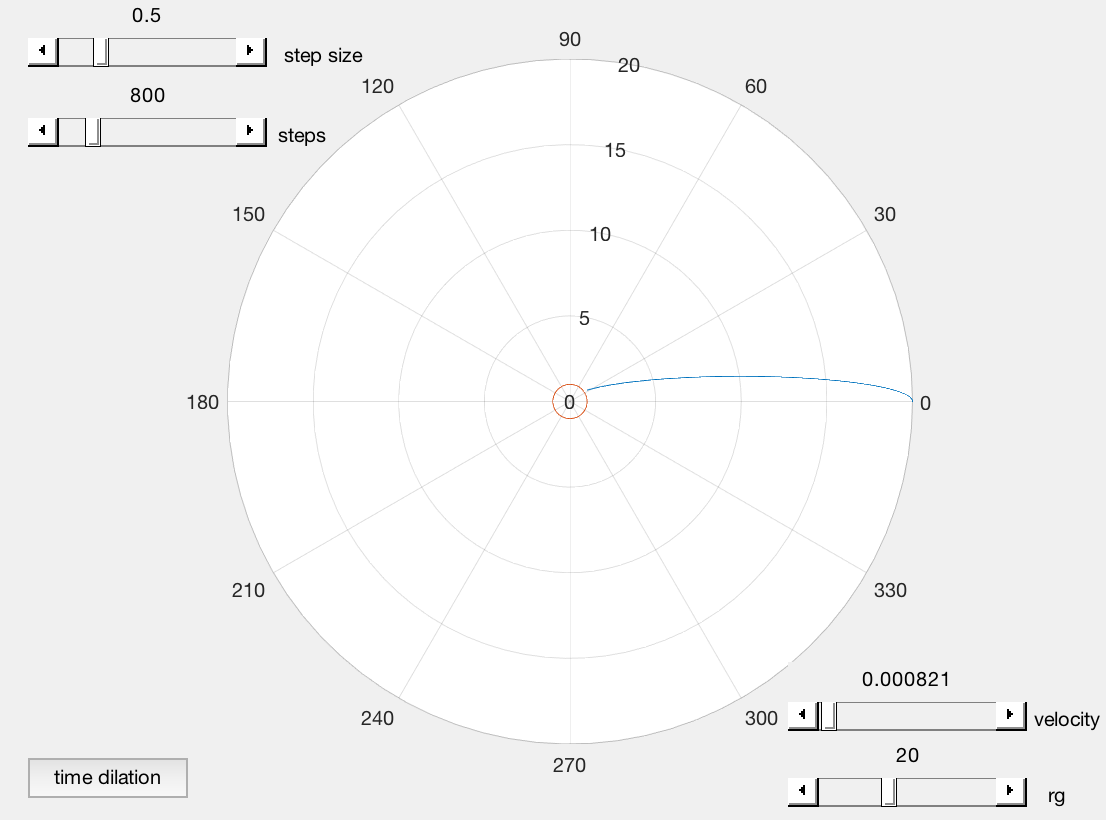
\includegraphics[width=12cm]{zeitreisen/gui.png}
        \caption{Grafische Benutzeroberfläche der Simulation}
        \label{skript:zeitreisen:fig:gui} 
    \end{figure}
    
    Das GUI beinhaltet einen polaren Plot der Geodäte, sowie zwei Schieber zum verändern von Startradius und Startgeschwindigkeit. Bei jeder Änderung dieser Werte wird im \texttt{myui.m} File die Funktion \texttt{update} aufgerufen, 
     \lstinputlisting[style=Matlab]{zeitreisen/listings/update.m} 
    welche die Berechnung neu startet und den Inhalt des Fensters aktualisiert.
    
    \subsection{Zeitdilation anzeigen}
    Im Fenster \ref{skript:zeitreisen:fig:gui} ganz unten links befindet sich der Knopf \texttt{time dilation}. Dieser ruft das Fenster \ref{skript:zeitreisen:fig:time} auf. In diesem sieht man nebst dem Verlauf der Winkelgeschwindigkeit (unten) auch die Änderungsrate der Zeit ($\dot{t}$, in der Mitte) und die aufsummierte Differenz der Eigenzeit zur Koordinatenzeit (time difference, zuoberst).
    
    Die oberen zwei Graphen sind wie folgt zu deuten. 
    
    Der mittlere Graph entspricht der Änderungsrate der Zeit zu jedem Zeitpunkt. Die x-Achse stellt dabei die Zeit für einen weit entfernten Beobachter dar. Sie ist direkt proportional zur Winkelgeschwindigkeit unten. Dies lässt sich einfach erklären. Je näher man am schwarzen Loch ist, desto höher ist die Änderungsrate der Zeit und die Beschleunigung, welche man erfährt. An ``Orten'' oder besser gesagt, an Abständen zum schwarzen Loch, an denen die Zeitänderung gross ist, ist man also nur kurz. Denn durch die starke Beschleunigung und die damit entstehenden Fliehkräfte vergrössert sich der Abstand schnell wieder.
    Dies ist natürlich nur der Fall, wenn der Raumfahrer nicht ins schwarze Loch abstürzt.
    
    Im oberen Graphen sieht man die Differenz der Zeit des Reisenden zur Koordinatenzeit. Sie steigt logischerweise streng monoton. In grosser Nähe zum schwarzen Loch, also an Orten mit grosser Winkelgeschwindigkeit und Zeitänderungsrate steigt sie steil. Da man sich an diesen Orten nur kurz befindet, flacht die Kurve danach jeweils schnell wieder ab. Der Endpunkt entspricht der total aufsummierten Differenz der Eigenzeit zur Koordinatenzeit. Er zeigt also direkt an, wie viele Sekunden man in die Zukunft gereist ist.
      \begin{figure}
        \centering
        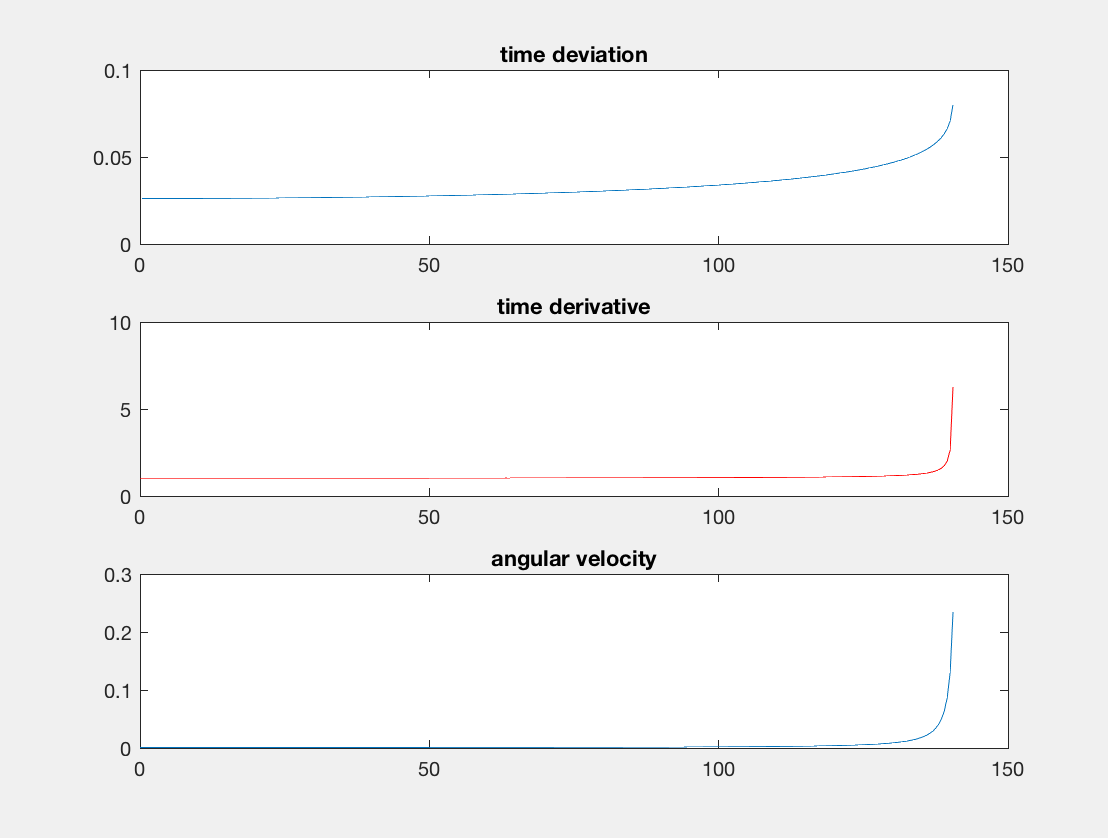
\includegraphics[width=12cm]{zeitreisen/time.png}
        \caption{Fenster für die Zeitänderung und Winkelgeschwindigkeit}
        \label{skript:zeitreisen:fig:time} 
    \end{figure}
    
    \subsection{Bedienung}
    
    Zum Schluss einige Bemerkungen zur Bedienung und ein Beispiel. 
    Die Regler für den Abstand ist auf Schwarzschild-Radien normiert. $20\,rg$ entsprechen also $20$ Schwarzschild-Radien Startabstand. Dadurch ist die Simulation für verschiedene schwarze Löcher gültig und der Schwarzschild-Radius muss nicht jedes Mal eingegeben werden.
    
    Die Wahl der Geschwindigkeit ist etwas heikel. Die maximale Geschwindigkeit wurde auf 30\%c festgelegt. Dies kann jedoch im Sourcecode geändert werden. Kleine Bewegungen am Schieber können grosse Auswirkungen haben. Am besten wählt man einen gewünschten Abstand und spielt mit der Geschwindigkeit, bis sich schöne Bahnen ergeben. Geraden deuten meistens darauf hin, dass die Geschwindigkeit zu gross war und man das schwarze Loch passiert hat.
    
    Zu tiefe Geschwindigkeiten führen zum Absturz ins schwarze Loch. Erkennbar daran, dass der Graph den orangen Ereignishorizont berührt oder an der Anzahl ungültiger Integrationen in der Kommandozeile. Dies lässt sich durch das Erhöhen der Geschwindigkeit leicht ausbessern.
    
    Die beiden Schieber oben links dienen der Genauigkeit und der Anzahl Schritte. Mit genügend Rechenleistung kann die Genauigkeit bis an den linken Anschlag vergrössert werden. Die Anzahl Schritte verlängert die Zeitreise. Je nach Abstand kann dies in einem Absturz enden. Die meisten Bahnen stürzen früher oder später ab. Nummerische Lösungen verschieben sich mit der Zeit etwas und kommen so dem Ereignishorizont zu nahe.
    
    Die Abbildung \ref{skript:zeitreisen:fig:Bsp} zeigt ein Beispiel für eine Geodäte sehr nahe dem schwarzen Loch.
      \begin{figure}
        \centering
        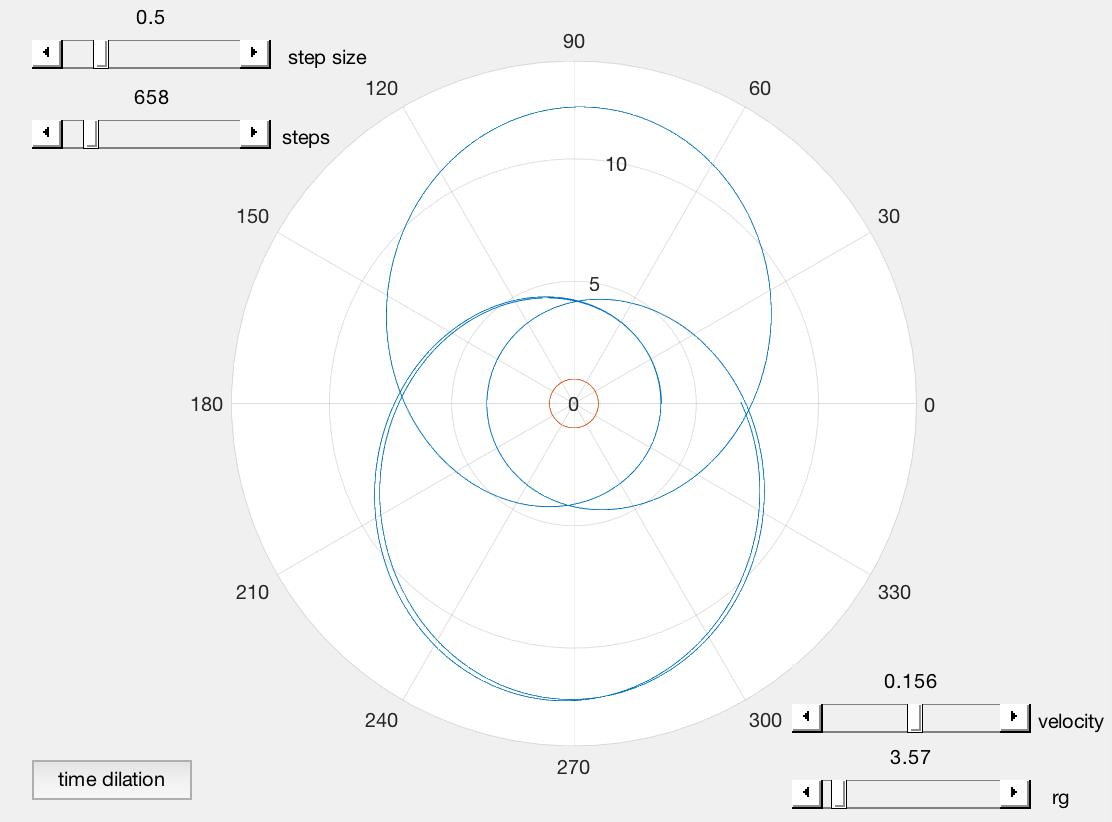
\includegraphics[width=12cm]{zeitreisen/Bsp.png}
        \caption{Beispiel für eine nahe Geodäte}
        \label{skript:zeitreisen:fig:Bsp} 
    \end{figure}
    \ref{skript:zeitreisen:fig:Bsp_time} zeigt den dazugehörigen Verlauf der Eigenzeit.
      \begin{figure}
        \centering
        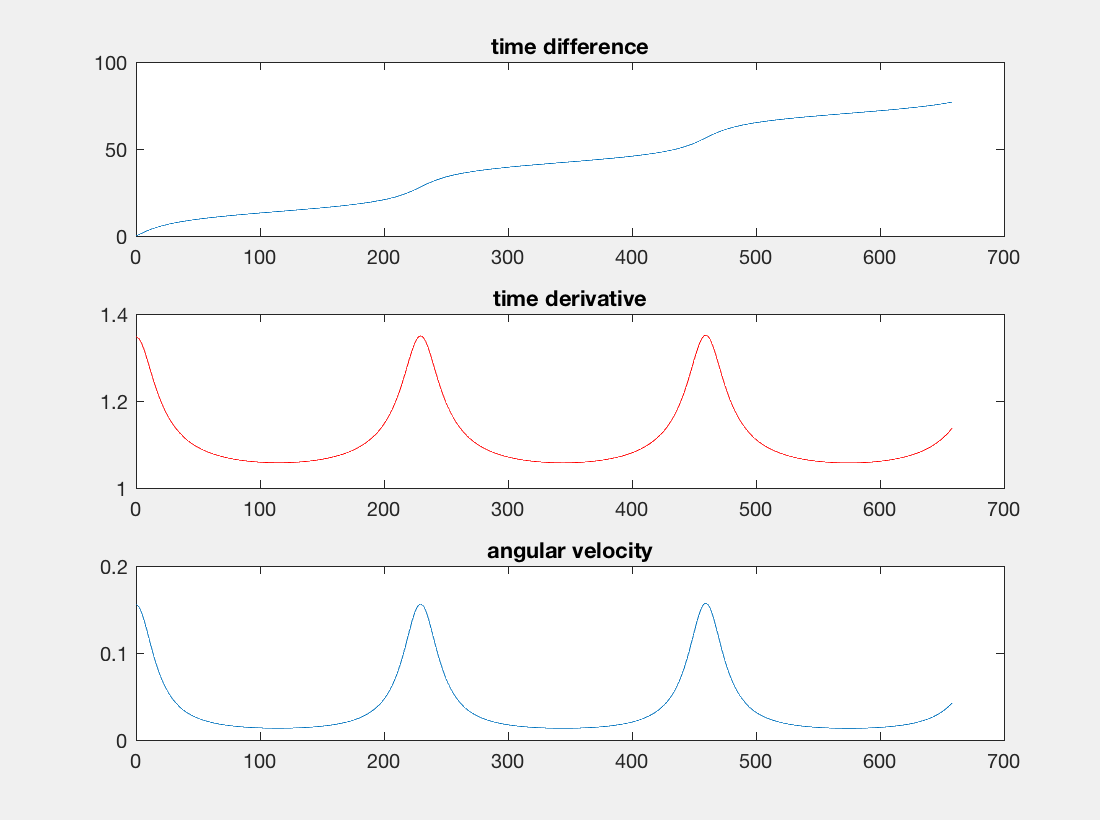
\includegraphics[width=12cm]{zeitreisen/Bsp_time.png}
        \caption{Verlauf der Eiegenzeit für Geodäte aus Bild \ref{skript:zeitreisen:fig:Bsp} }
        \label{skript:zeitreisen:fig:Bsp_time} 
    \end{figure}
    Man sieht deutlich, dass der Reisende nahe dem schwarzen Loch eine starke Beschleunigung erfährt. Nach rund $735$ Sekunden in Koordinatenzeit vergingen für den Reisenden bloss $658$ Sekunden. Er ist also eine Minute und $17$ Sekunden in die Zukunft gereist. Das entspricht einem Gewinn von ca. $10\%$.
    
   	\section{Fazit}
    \rhead{Fazit}
    
    Zeitreisen sind also möglich, sofern sie die Zukunft betreffen. Sowohl theoretisch als auch praktisch lassen sich diese Effekte nachweisen. Wir haben gesehen, dass Gravitation und Geschwindigkeit solche Reisen ermöglichen.
    
    Sind damit nun grosse Zeitreisen möglich? Solche wie sie uns etwa im Film Interstellar versprochen werden? Dort Reisen die Hauptdarsteller in einer Stunde $7$ Jahre in die Zukunft. Die Antwort lautet nein. Die grössten Probleme gibt es bezüglich der Realisierbarkeit. Der Mensch erreicht einfach nicht eine genug hohe Geschwindigkeit, um weit entfernte supermassive schwarze Löcher zu erreichen oder genug von der Zeitdilatationswirkung zu profitieren. Die benötigte Energie für so ein Vorhaben wäre ebenfalls immens.
    
    Ein anderes Problem stellt die Verwendung von Geodäten dar. Um nicht noch mehr Energie für Steuerdüsen verwenden zu müssen, entschieden wir uns für diese. Dadurch sind wir aber jeweils nur kurz dem schwarzen Loch nahe, wenn wir einen Absturz vermeiden wollen. Die Zeitgewinnung wird dadurch kleiner. Man müsste länger und näher bei einem schwarzen Loch verharren können, um wirklich davon zu profitieren. 
    
    Mit der Schwarzschild-Metrik konnten wir also Zeitreisen beschreiben. Allerdings ist deren Einfluss auf die Zeit für Film-ähnliche Effekte zu klein. Es bleibt zu prüfen, ob unter Verwendung der Kerr-Metrik grössere Effekte auftreten \dots
        
	\printbibliography[heading=subbibliography]
	\end{refsection}

